\documentclass[aspectratio=169]{beamer}
\usepackage{amsmath,booktabs,graphicx}
\usetheme{Madrid}

\setbeamertemplate{navigation symbols}{} % Remove navigation icons

\begin{document}

% --- Anushka --- %
% --- Slide 0: Title --- %
\begin{frame}
    \begin{center}
        \vspace{0.8cm}
        {\LARGE \textbf{Enabling Differential Privacy}}\\[0.5cm]
        {\large in HPE's Swarm Learning}\\[0.8cm]
        \rule{7cm}{0.4pt}\\[0.5cm]
        {\normalsize Anushka \quad | \quad Sidharth \quad | \quad Hima \quad | \quad Allen \quad | \quad Goutham }\\[0.3cm]
    \end{center}
\end{frame}

% --- Slide 1: What is Swarm Learning? ---
\begin{frame}{What is Swarm Learning?}
    \begin{columns}[T]
        \begin{column}{0.55\textwidth}
            \begin{block}{Definition}
                \textbf{HPE Swarm Learning} is a decentralized, privacy-preserving ML framework that uses computing power at distributed data sources to train models — without sharing raw data. Collaboration is secured via a \textbf{blockchain} platform.
            \end{block}
            \vspace{0.3cm}
            \textbf{How it differs from standard FL}
            \begin{itemize}
                \item No central server — fully peer-to-peer
                \item Training occurs at the \textbf{edge}, where data lives
                \item Only model weights are shared; \textbf{raw data never leaves} the node
            \end{itemize}
        \end{column}
        \begin{column}{0.45\textwidth}
            \includegraphics[width=\textwidth]{why_swarm.png}
        \end{column}
    \end{columns}
\end{frame}

\begin{frame}{Swarm Network Architecture}
    \begin{center}
        \includegraphics[width=0.5\textwidth]{swarm_components.png}
    \end{center}
\end{frame}

% --- Slide 2: Swarm Network Components (1/2) ---
\begin{frame}{Node Types in a Swarm Network}
    \begin{columns}[T]
        \begin{column}{0.48\textwidth}
            \begin{block}{SL Node (Swarm Learning Node)}
                \begin{itemize}
                    \item Core ML training component
                    \item Trains locally on private data
                    \item Shares model weights with peers; never raw data
                    \item Merges insights received from other SL nodes
                \end{itemize}
            \end{block}
        \end{column}
        \begin{column}{0.48\textwidth}
            \begin{block}{SN Node (Swarm Network Node)}
                \begin{itemize}
                    \item Forms the Ethereum blockchain network
                    \item Maintains training state and coordinates the swarm
                    \item Stores only metadata — \textit{not} model weights
                \end{itemize}
            \end{block}
        \end{column}
    \end{columns}
\end{frame}

% --- Slide 3: Swarm Network Components (2/2) ---
\begin{frame}{Node Types in a Swarm Network (contd.)}
    \begin{columns}[T]
        \begin{column}{0.48\textwidth}
            \begin{block}{Sentinel Node}
                \begin{itemize}
                    \item A special SN node that initializes the blockchain
                    \item Must be the first node to start in any swarm run
                    \item Blockchain state can persist across restarts
                \end{itemize}
            \end{block}
        \end{column}
        \begin{column}{0.48\textwidth}
            \begin{block}{SWOP \& SWCI}
                \begin{itemize}
                    \item \textbf{SWOP:} Operator agent — starts/stops runs, builds and upgrades ML containers
                    \item \textbf{SWCI:} Command interface — connects to SN nodes for monitoring and management
                \end{itemize}
            \end{block}
        \end{column}
    \end{columns}
\end{frame}

% --- Slide 4: How Swarm Training Works ---
\begin{frame}{The Swarm Training Loop}
    \begin{columns}[T]
        \begin{column}{0.55\textwidth}
            \begin{enumerate}
                \item \textbf{Acquire identity:} Each SL node obtains an X.509/SPIRE certificate and a license.
                \item \textbf{Register:} Node registers with an SN node and starts its local file server.
                \item \textbf{Train locally:} Nodes train independently on their private data.
                \item \textbf{Synchronize:} At set intervals, nodes share model updates — not raw data — with peers.
                \item \textbf{Leader election:} One node is elected \textit{Leader} to aggregate all updates.
                \item \textbf{Merge \& distribute:} Leader produces a global model and sends it back to all nodes.
            \end{enumerate}
        \end{column}
        \begin{column}{0.42\textwidth}
            \begin{block}{Minimum Peers}
                \begin{itemize}
                    \item A minimum peer count can be set for synchronization
                    \item Sync is blocked if peers fall below this threshold
                    \item Resumes once enough peers reach the sync point
                \end{itemize}
            \end{block}
        \end{column}
    \end{columns}
\end{frame}

% --- Slide 5: Synchronization ---
\begin{frame}{Controlling Synchronization Frequency}
    \begin{columns}[T]
        \begin{column}{0.48\textwidth}
            \begin{block}{Sync Frequency}
                \begin{itemize}
                    \item Determines how often nodes share updates
                    \item Measured in training batches
                    \item Large value $\rightarrow$ fewer synchronizations, faster training
                    \item Small value $\rightarrow$ more synchronizations, better accuracy
                \end{itemize}
            \end{block}
        \end{column}
        \begin{column}{0.48\textwidth}
            \begin{block}{Adaptive Synchronization}
                \begin{itemize}
                    \item Adjusts sync frequency automatically based on training signal
                    \item Loss decreasing $\rightarrow$ synchronize less often
                    \item Loss stagnant $\rightarrow$ synchronize more often
                \end{itemize}
            \end{block}
        \end{column}
    \end{columns}
\end{frame}

% --- Slide 6: Model Merging ---
\begin{frame}{Model Merging and Merge Methods}
    \begin{columns}[T]
        \begin{column}{0.48\textwidth}
            \begin{block}{How it works}
                \begin{itemize}
                    \item One SL node is elected \textbf{Leader}
                    \item Leader collects model updates from all peers
                    \item Creates a single global model
                    \item Sends the merged model back to all nodes
                    \item Each node uses the merged model to start the next training batch
                \end{itemize}
            \end{block}
        \end{column}
        \begin{column}{0.48\textwidth}
            \begin{block}{Merge Methods}
                \begin{itemize}
                    \item \textbf{Mean} (Federated Averaging) — default; weighted average of all updates
                    \item \textbf{Coordinate Median} — uses the median instead of mean; robust against outliers
                    \item \textbf{Geometric Median} — uses Weiszfeld's algorithm; better represents all nodes
                \end{itemize}
            \end{block}
        \end{column}
    \end{columns}
\end{frame}

% --- Slide 7: Leader Failure & Model Exchange ---
\begin{frame}{Leader Failure Detection and Recovery (LFDR)}
    \begin{columns}[T]
        \begin{column}{0.48\textwidth}
            \begin{alertblock}{When the Leader Fails}
                \begin{itemize}
                    \item If the leader fails \textit{during} the merge process, training does not halt
                    \item A new leader is automatically elected to continue merging
                    \item If the failed leader recovers, it rejoins as a normal SL node
                \end{itemize}
            \end{alertblock}
        \end{column}
        \begin{column}{0.48\textwidth}
            \begin{block}{Model Exchange}
                \begin{itemize}
                    \item Each SL node uses the merged model to begin the next training batch
                    \item Exchange is coordinated by the SN network
                    \item Models are transferred via the Swarm Learning file server
                \end{itemize}
            \end{block}
        \end{column}
    \end{columns}
\end{frame}

% --- Sidharth --- %
% --- Slide 1: The Swarm Privacy Paradox ---
\begin{frame}{The Privacy Paradox in Swarm Learning}
    \begin{center}
        \large{\textbf{``Decentralization $\neq$ Absolute Privacy''}}
    \end{center}
    \vspace{0.3cm}

    While Swarm Learning eliminates the single point of failure (central server) and keeps raw data $D_i$ localized at edge nodes, it introduces a severe vector of indirect vulnerability.

    \begin{block}{The Underlying Mechanism of Leakage}
        During P2P consensus stages, nodes broadcast intermediate model parameters $\theta_i$ or gradient updates $\nabla L(\theta_i)$. These weights contain high-dimensional mathematical footprints of the underlying local private distributions.
    \end{block}

    \begin{alertblock}{The Problem}
        An adversary monitoring the blockchain state channels or interacting as an honest-but-curious peer can reverse-engineer private local data directly from public model parameters.
    \end{alertblock}
\end{frame}

% --- Slide 2: Adversarial Threat Model & Attacks ---
\begin{frame}{The Threat Model: Attack Vectors on Swarm Nodes}
    We assume an ecosystem where malicious or compromised nodes have access to shared peer parameters $\theta$ over the peer-to-peer network layer.

    \vspace{0.3cm}
    \begin{table}[]
        \centering
        \small
        \begin{tabular}{p{3.5cm} p{4.5cm} p{4.5cm}}
            \toprule
            \textbf{Attack Type} & \textbf{Mechanism} & \textbf{Impact on Swarm Node} \\
            \midrule
            \textbf{Gradient Inversion} & Reconstructing inputs $x$ from public gradients $\nabla L(\theta_i)$. & Complete exposure of training images/clinical records. \\
            \addlinespace
            \textbf{Membership Inference (MIA)} & Determining if target record $x \in D_i$ based on model confidence spikes. & Breach of individual data presence confidentiality. \\
            \addlinespace
            \textbf{Generative Adversarial Leakage (GAN)} & Malicious peer acts as a generator, utilizing shared $\theta$ as a discriminator. & Reconstruction of high-fidelity synthetic client datasets. \\
            \bottomrule
        \end{tabular}
    \end{table}
\end{frame}

% --- Slide 3: Practical Barriers of Standard DP ---
\begin{frame}{The Double Bottleneck of Standard Differential Privacy}
    While Differential Privacy (DP) mathematically thwarts parameter reverse-engineering, applying standard DP algorithms over a standard federated training loop presents major bottlenecks:

    \begin{columns}[T]
        \begin{column}{0.48\textwidth}
            \begin{alertblock}{1. Permanent Metric Degradation}
                \begin{itemize}
                    \item Model accuracy and overall quality drop severely compared to non-DP baselines.
                    \item \textbf{No Epoch Cure:} This accuracy gap is structural; it \textbf{cannot} be resolved by simply running more training epochs due to cumulative noise effects.
                \end{itemize}
            \end{alertblock}
        \end{column}
        
        \begin{column}{0.48\textwidth}
            \begin{alertblock}{2. Computation \& Latency Penalty}
                \begin{itemize}
                    \item Total training time increases by at least \textbf{2X or more}.
                    \item Exact execution latency depends highly on the chosen framework, batch configurations, and DP-specific optimization arguments.
                \end{itemize}
            \end{alertblock}
        \end{column}
    \end{columns}

    \vspace{0.3cm}
    \begin{center}
        \textit{We face a zero-sum trade-off: stronger mathematical privacy inherently destroys utility and runtime efficiency.}
    \end{center}
\end{frame}

% --- Slide 4: The Proposed Cascaded Swarm Learning Solution ---
\begin{frame}{Proposed Solution: Cascaded P2P Swarm Ensemble}
    To break this trade-off, a \textbf{Cascaded Ensemble of Swarm Learning} is executed in two distinct, sequential phases:

    \vspace{0.3cm}
    \begin{columns}[T]
        \begin{column}{0.48\textwidth}
            \begin{block}{Round 1: The Secure Anchor (With DP)}
                \begin{itemize}
                    \item \textbf{Execution:} Swarm Learning with active DP.
                    \item \textbf{Setup:} Run on a minimal, highly curated subset of data for a small number of epochs.
                    \item \textbf{Outcome:} Establishes a robust, structurally generic initial model without exhausting the privacy budget.
                \end{itemize}
            \end{block}
        \end{column}

        \begin{column}{0.48\textwidth}
            \begin{block}{Round 2: The Utility Refiner (Without DP)}
                \begin{itemize}
                    \item \textbf{Execution:} Standard Swarm Learning (Non-DP).
                    \item \textbf{Setup:} Run on the full dataset with a higher number of training epochs.
                    \item \textbf{Outcome:} Uses the Round 1 model as a secure, pre-trained starting point to recover validation accuracy.
                \end{itemize}
            \end{block}
        \end{column}
    \end{columns}
\end{frame}


% --- Allen --- %
%--------------------------------------------------
% Slide 1: Motivation & Concept
%--------------------------------------------------
\begin{frame}{Cascaded Differential Privacy: The Big Idea}
\begin{alertblock}{The Problem with Full‑DP}
Applying DP throughout \emph{all} training epochs:
\begin{itemize}
    \item Degrades model accuracy (noise accumulation).
    \item Slows training (2×–10× overhead from clipping/noise).
    \item Exhausts the privacy budget $\varepsilon$ with diminishing returns.
\end{itemize}
\end{alertblock}

\pause
\begin{exampleblock}{Cascaded DP Solution}
\begin{itemize}
    \item \textbf{Phase 1}: Train with DP-Adam (strong privacy) \emph{only until convergence}.
    \item \textbf{Phase 2}: Disable DP, switch to standard optimizer (Adam) to recover accuracy.
    \item Decentralised swarm‑wide vote determines the transition point.
\end{itemize}
\end{exampleblock}
\end{frame}

%--------------------------------------------------
% Slide 2: Two Phases Illustrated
%--------------------------------------------------
\begin{frame}{Two Distinct Training Phases}
\begin{columns}[T]
\column{0.48\textwidth}
\begin{block}{Phase 1: Privacy‑Preserving}
\begin{itemize}
    \item DP-Adam (noisy, clipped gradients).
    \item Convergence monitoring: gradient norm + validation accuracy.
    \item Swarm nodes vote when their local model stabilises.
    \item DP \textbf{ON} – protects against gradient leakage.
\end{itemize}
\end{block}

\column{0.48\textwidth}
\begin{block}{Phase 2: Performance Recovery}
\begin{itemize}
    \item Standard Adam (no DP noise).
    \item Full gradient information for fine‑tuning.
    \item No further $\varepsilon$ consumption.
    \item Model accuracy rebounds toward non‑private baseline.
\end{itemize}
\end{block}
\end{columns}
\end{frame}

%--------------------------------------------------
% Slide 3: Convergence Criteria (How to Decide “When”)
%--------------------------------------------------
\begin{frame}{How a Node Decides It’s Time to Drop DP}
Each node monitors two metrics over a rolling window ($W=5$ epochs):

\vspace{0.3cm}
\begin{columns}[t]
\column{0.5\textwidth}
\textbf{Gradient Norm Stabilisation}
\[
\left|\frac{\text{norm}_t - \overline{\text{norm}}_{\text{roll}}}
           {\overline{\text{norm}}_{\text{roll}}}\right| 
           < \theta_g \quad (\text{e.g. } 2\%)
\]

\column{0.5\textwidth}
\textbf{Validation Accuracy Plateau}
\[
\mathrm{Var}(\text{acc}_{\text{roll}}) 
    < \theta_a \quad (\text{e.g. } 0.5\%)
\]
\end{columns}

\vspace{0.4cm}
\begin{itemize}
    \item Both conditions must hold simultaneously.
    \item A \texttt{MIN\_DP\_EPOCHS} guard prevents premature disabling.
    \item Alternative: SNR‑based detection (gradient norm / $\sigma_{\text{eff}}$) – more adaptive.
\end{itemize}
\end{frame}

%--------------------------------------------------
% Slide 4: Swarm Consensus & Transition
%--------------------------------------------------
\begin{frame}{Decentralised Vote and Cascaded Transition}
\begin{enumerate}
    \item A node that meets convergence criteria \textbf{casts a vote}.
    \item Votes shared via a common scratch space (e.g., shared file, blockchain event).
    \item DP remains active until \textbf{all} participating nodes have voted.
    \item Once quorum is reached:
    \begin{itemize}
        \item DP is disabled simultaneously across the swarm.
        \item The DP‑optimiser is replaced with a standard optimiser.
    \end{itemize}
\end{enumerate}

\vspace{0.3cm}
\begin{block}{Why wait for all nodes?}
    Prevents a fast‑converging node from exposing the swarm prematurely.  
    Ensures every data owner’s privacy is protected until their own data is no longer at risk.
\end{block}
\end{frame}

%--------------------------------------------------
% Slide 5: Voting Diagram
%--------------------------------------------------
\begin{frame}{Swarm‑Wide DP Drop Voting Procedure}
\centering
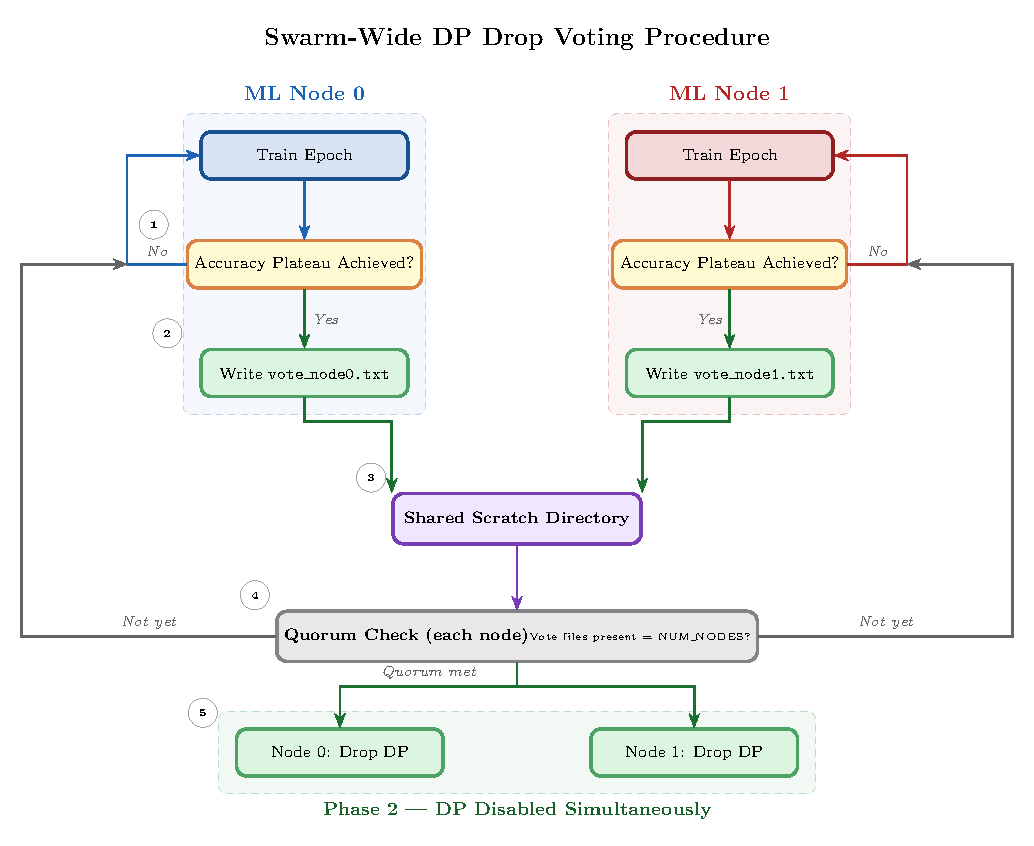
\includegraphics[width=0.80\textwidth,height=0.85\textheight]{voting_diagram.pdf}
\end{frame}

%--------------------------------------------------
% Slide 6: Benefits & Expected Results
%--------------------------------------------------
\begin{frame}{Why Cascaded DP Outperforms Full DP}
\begin{center}
\begin{tabular}{@{}lccc@{}}
\toprule
\textbf{Metric}           & \textbf{No DP} & \textbf{Full DP} & \textbf{Cascaded DP} \\
\midrule
Privacy Protection        & None           & Strong            & Strong (early phase) \\
Final Accuracy            & High           & Moderate / Low    & \textbf{High (recovers)} \\
Training Time             & Fast           & Slow (2–10×)      & \textbf{Fast (majority)} \\
$\varepsilon$ Consumption & 0              & High              & \textbf{Low} \\
\bottomrule
\end{tabular}
\end{center}

\vspace{0.3cm}
\begin{itemize}
    \item Cascaded DP retains the privacy guarantee during the most vulnerable early epochs.
    \item The model recovers accuracy and speeds up once DP is removed.
    \item Total privacy budget consumed is dramatically reduced.
\end{itemize}
\end{frame}


% --- Hima --- Results --- %
%--------------------------------------------------
% Results Slide 1: Accuracy Breakdown (alpha = 1.0)
%--------------------------------------------------
\begin{frame}{Results: Accuracy Recovery Under CascadedDP ($\alpha = 1.0$)}
\centering
\includegraphics[width=0.72\textwidth]{results_section/accuracy_breakdown_bar.png}
\end{frame}

%--------------------------------------------------
% Results Slide 2: Observations on Accuracy Breakdown
%--------------------------------------------------
\begin{frame}{Key Observations: Accuracy Breakdown}
\begin{itemize}
    \item CascadedDP closes most of the privacy--utility gap: the final test accuracy of \textbf{87.94\%} sits within 0.5 points of the No~DP baseline (\textbf{88.44\%}), versus a 5.5-point gap for Full~DP (\textbf{82.93\%}).
    \item The Stage~1 dip to \textbf{77.50\%} reflects the cost of active DP noise during the privacy-protected phase (epochs 1--12) -- this is the expected, bounded trade-off, not a failure mode.
    \item Stage~2 shows the model recovering sharply once DP is dropped, climbing from 77.50\% to \textbf{85.47\%} on validation and \textbf{87.94\%} on the held-out test set.
    \item This confirms the core hypothesis: stabilized gradients before the drop point imply diminishing marginal sensitivity, so continued DP overhead after convergence is unjustified.
\end{itemize}
\end{frame}

%--------------------------------------------------
% Results Slide 3: Runtime Breakdown (alpha = 1.0)
%--------------------------------------------------
\begin{frame}{Results: Runtime Savings Under CascadedDP ($\alpha = 1.0$)}
\centering
\includegraphics[width=0.65\textwidth,height=0.82\textheight,keepaspectratio]{results_section/runtime_breakdown_bar.png}
\end{frame}

%--------------------------------------------------
% Results Slide 4: Observations on Runtime Breakdown
%--------------------------------------------------
\begin{frame}{Key Observations: Runtime Breakdown}
\begin{itemize}
    \item CascadedDP completes training in \textbf{673s} total, a \textbf{40\% reduction} versus Full~DP's \textbf{1130s} -- while only adding \textbf{29\%} over the No~DP baseline of \textbf{520s}.
    \item Only \textbf{266s} (Stage~1) are spent under DP-Adam overhead; the remaining \textbf{407s} (Stage~2) run at standard-optimizer speed.
    \item Because the DP-active window is short and bounded by the convergence trigger -- not a fixed fraction of total epochs -- the runtime penalty does not scale linearly with training length.
    \item Net effect: most of the wall-clock cost of DP is paid once, early, and is never repeated for the remaining epochs.
\end{itemize}
\end{frame}

%--------------------------------------------------
% Results Slide 4b: Validation Accuracy vs Epoch (New Table)
%--------------------------------------------------
\begin{frame}{CascadedDP Stage 1: Late-Epoch Validation Progression}
\vspace{0.2cm}
\begin{columns}[v]
\begin{column}{0.48\textwidth}
    \centering
    \small
    \begin{tabular}{cc}
        \toprule
        \textbf{Epoch} & \textbf{Validation Accuracy (\%)} \\ \midrule
        8              & 74.35                             \\
        9              & 75.56                             \\
        10             & 76.01                             \\
        11             & 76.32                             \\
        \textbf{12 (Drop Point)} & \textbf{77.50}           \\ \bottomrule
    \end{tabular}
\end{column}
\hfill
\begin{column}{0.48\textwidth}
    \small
    \textbf{Context \& Dynamics:}
    \begin{itemize}
        \item Shows the steady ascent toward convergence right before the privacy block is dropped at Epoch 12.
        \item The final step up to \textbf{77.50\%} serves as the baseline starting point for the unconstrained Stage~2 recovery phase.
    \end{itemize}
\end{column}
\end{columns}
\end{frame}

%--------------------------------------------------
% Results Slide 5: Runtime vs. Data Heterogeneity
%--------------------------------------------------
\begin{frame}{Results: Runtime vs. Data Heterogeneity}
\centering
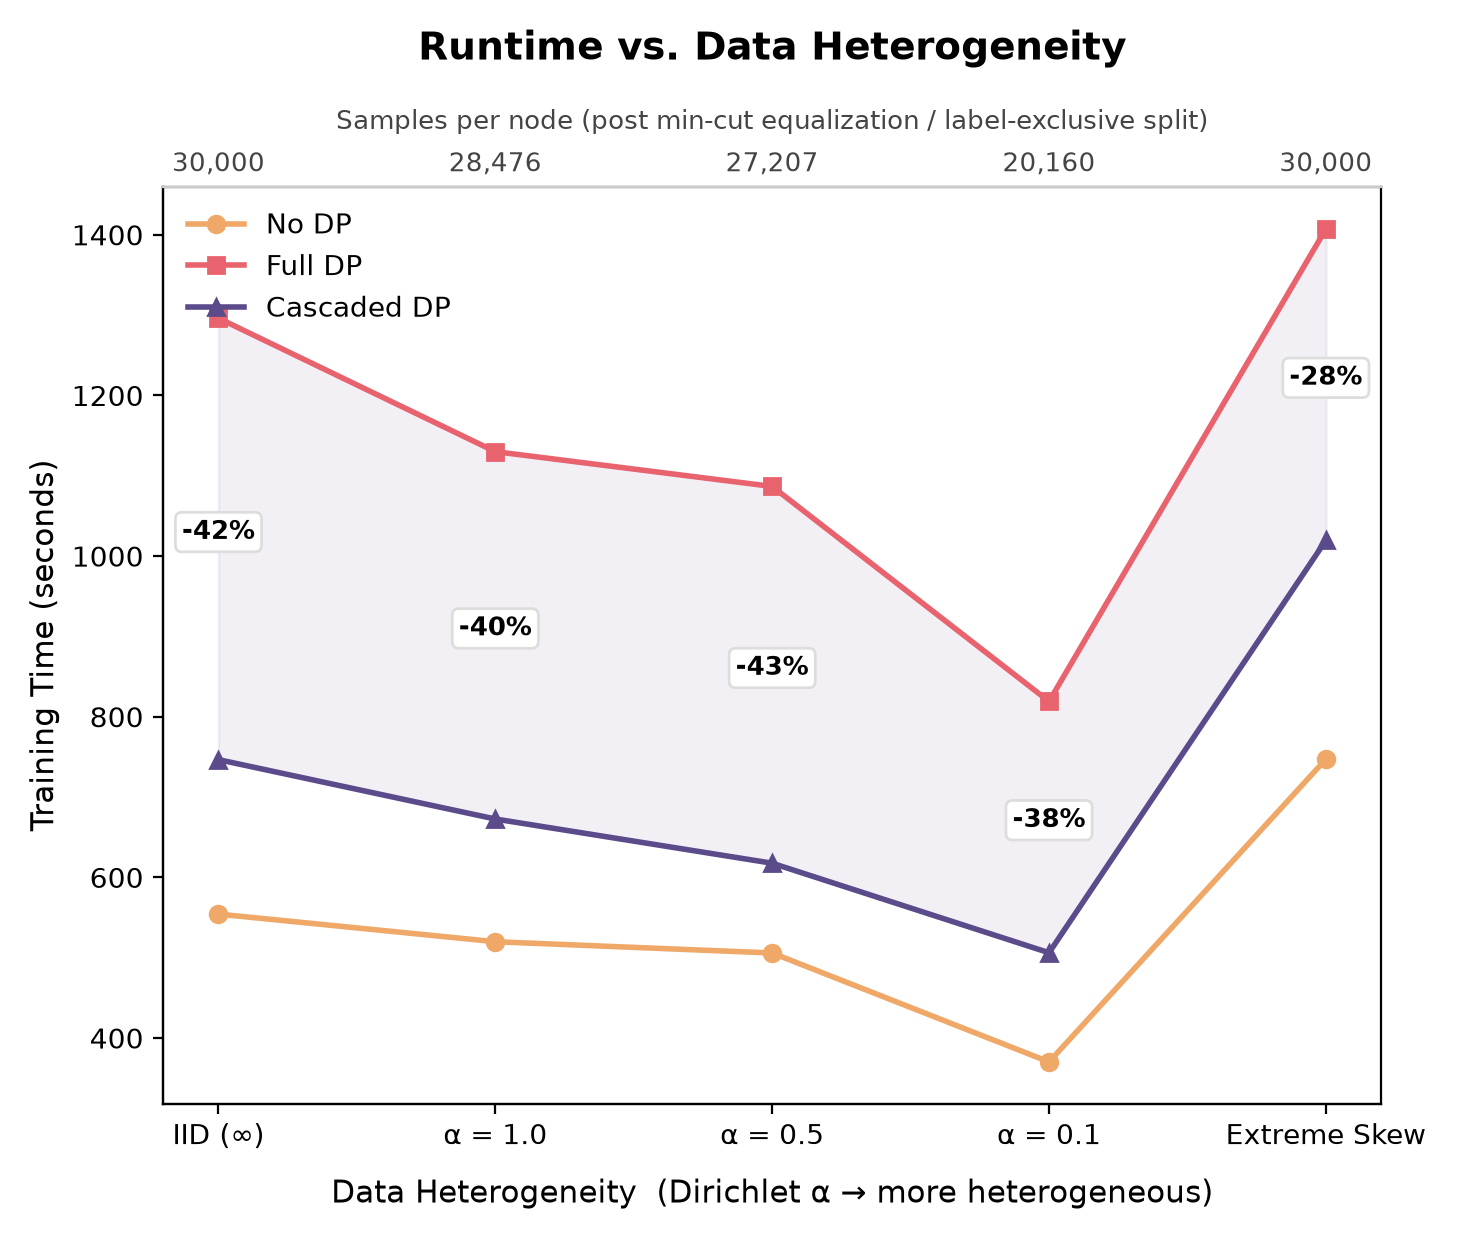
\includegraphics[width=0.78\textwidth,height=0.82\textheight,keepaspectratio]{results_section/runtime_vs_heterogeneity_twin_axis.png}
\end{frame}

%%--------------------------------------------------
% Results Slide 6: Observations on Runtime vs. Heterogeneity
%--------------------------------------------------
\begin{frame}{Key Observations: Runtime vs. Heterogeneity}
\begin{itemize}
    \item The CascadedDP-over-Full-DP runtime saving is consistently large and stable across the heterogeneity sweep: \textbf{42\%} (IID), \textbf{40\%} ($\alpha=1.0$), \textbf{43\%} ($\alpha=0.5$), \textbf{38\%} ($\alpha=0.1$), and \textbf{22\%} (Extreme Skew).
    \item Absolute runtimes fall toward $\alpha = 0.1$ for \emph{all three} methods -- this tracks the samples-per-node axis shown above the plot (\textbf{30{,}000 $\rightarrow$ 20{,}160}), a side effect of Dirichlet min-cut equalization, not heterogeneity itself.
    \item Because all three curves shrink together, the \emph{relative} CascadedDP advantage is preserved even though the \emph{absolute} numbers are confounded by shrinking dataset size at low $\alpha$.
    \item Extreme Skew uses a different, label-exclusive partitioning (5 classes/node, no Dirichlet trimming) and returns to full 30{,}000-sample volume -- explaining the runtime rebound at the right edge of the plot.
\end{itemize}
\end{frame}

%--------------------------------------------------
% Results Slide 7: Accuracy vs. Data Heterogeneity
%--------------------------------------------------
\begin{frame}{Results: Accuracy vs. Data Heterogeneity}
\centering
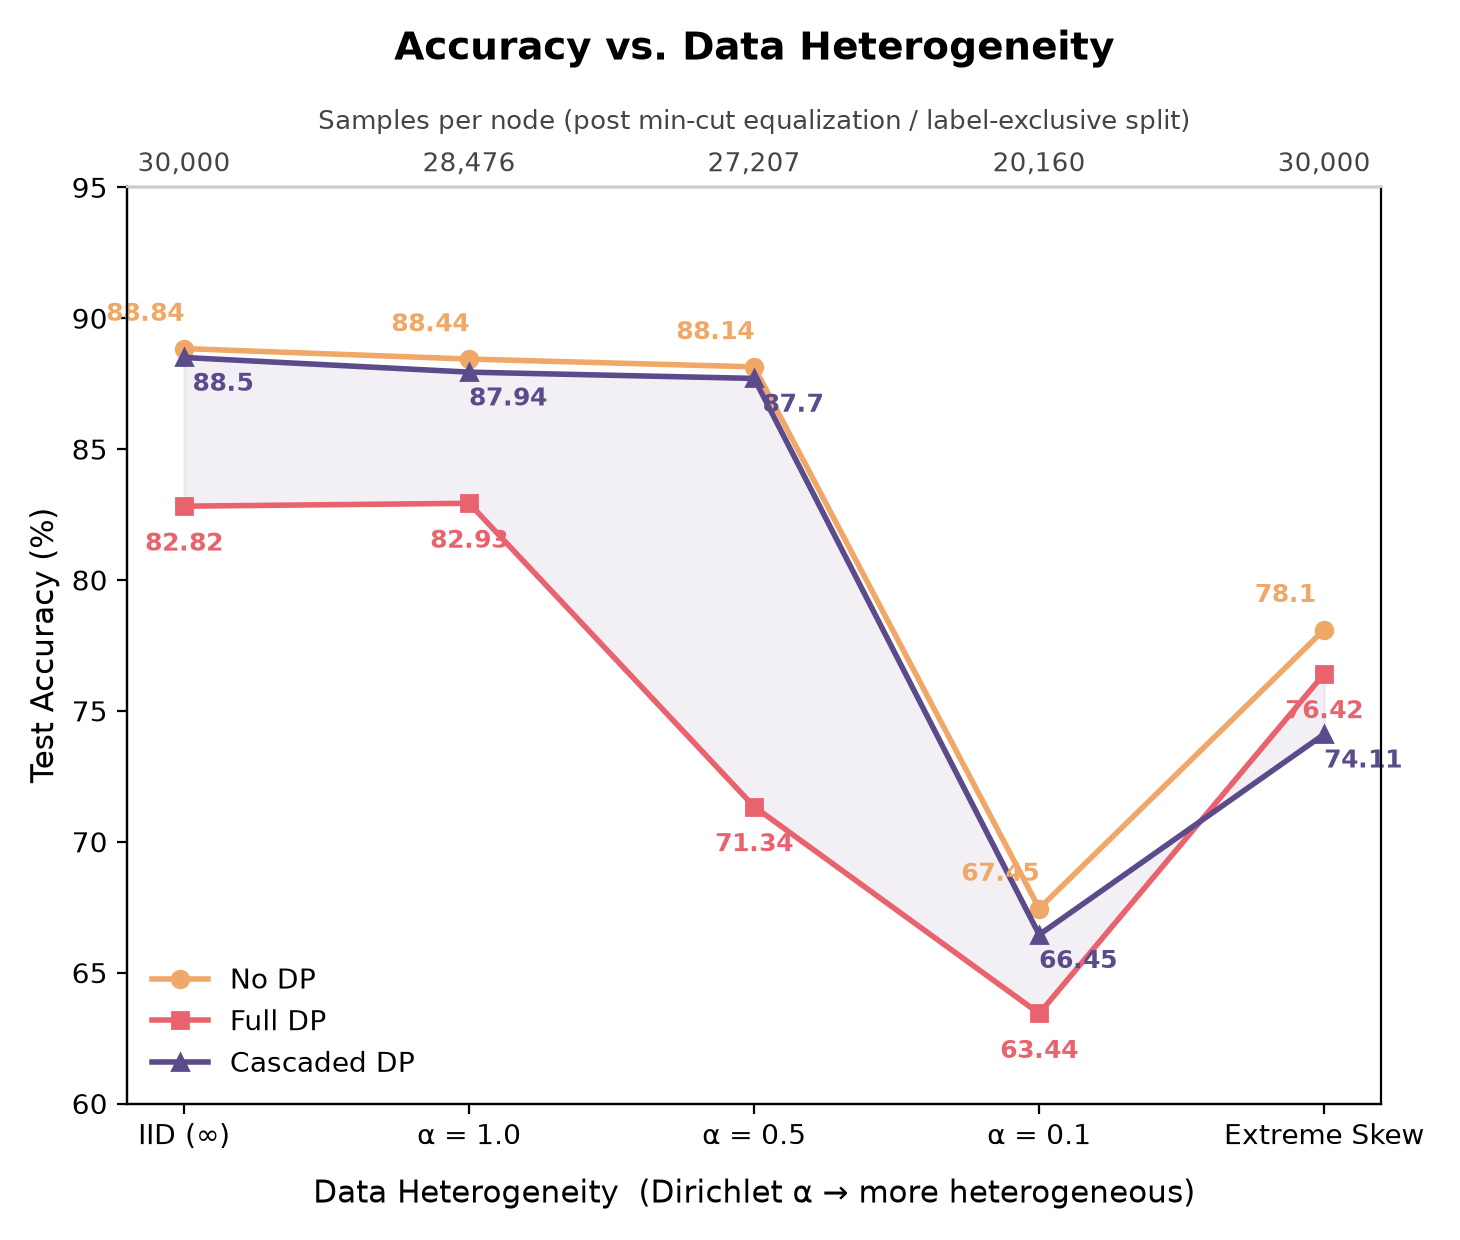
\includegraphics[width=0.78\textwidth,height=0.82\textheight,keepaspectratio]{results_section/accuracy_vs_heterogeneity_twin_axis.png}
\end{frame}

%--------------------------------------------------
% Results Slide 8: Observations on Accuracy vs. Heterogeneity
%--------------------------------------------------
\begin{frame}{Key Observations: Accuracy vs. Heterogeneity}
\begin{itemize}
    \item CascadedDP tracks the No~DP baseline closely from IID through $\alpha = 0.5$ (within 0.5 points), while Full~DP degrades sharply over the same range ($82.8\% \rightarrow 71.3\%$).
    \item All three methods drop together at $\alpha = 0.1$ -- this coincides with the smallest samples-per-node point (\textbf{20{,}160}), so part of this dip is a data-volume effect layered on top of heterogeneity, not heterogeneity alone.
    \item At Extreme Skew, CascadedDP (\textbf{75.43\%}) underperforms Full~DP (\textbf{77.26\%}) by a small margin (1.83\%), remaining close to the No~DP baseline (\textbf{77.43\%}). This might hint at an early convergence due to local gradients converging.
    \item Overall takeaway: CascadedDP's accuracy advantage over Full~DP is robust across realistic heterogeneity regimes ($\alpha \ge 0.5$), with a narrow trade-off profile discovered under maximal label skew.
\end{itemize}
\end{frame}
%--------------------------------------------------
% Results Slide 9: 2D Heterogeneity Matrix Plot
%--------------------------------------------------
\begin{frame}{Empirical Validation: 2D Heterogeneity Matrix}
\begin{center}
    \includegraphics[width=\textwidth,height=0.75\textheight,keepaspectratio]{results_section/matrix_graph.png}
\end{center}
\end{frame}
%--------------------------------------------------
% Results Slide 10: Analysis of Cross-Skew Profiles
%--------------------------------------------------
\begin{frame}{Deep Dive: Dissecting Partition Skews}
\begin{itemize}
    \item \textbf{Quantity Skew:} Mitigates straggler overhead; drops Full~DP peak runtime ($1639\,\text{s} \rightarrow 1016\,\text{s}$) while retaining $86.65\%$ accuracy.
    
    \item \textbf{Label Skew:} High standalone robustness; matches No~DP baseline accuracy ($88.28\%$ vs. $88.36\%$) and slashes runtime by $460\,\text{s}$ ($1179\,\text{s} \rightarrow 718\,\text{s}$).
    
    \item \textbf{Combined Skew:} Dual skew anomalies scale additively rather than compounding multiplicatively.
    
    \item \textbf{Core Takeaway:} Robust middle ground—remains within $1\text{--}2\%$ of the No~DP utility ceiling with a consistent $33\%\text{--}40\%$ runtime reduction over Full~DP.
\end{itemize}
\end{frame}
%--------------------------------------------------
% Conclusion Slide
%--------------------------------------------------
\begin{frame}{Conclusion \& Future Outlook}
\begin{block}{Breaking the Privacy--Utility Deadlock}
    Our evaluation of \textbf{CascadedDP} demonstrates that privacy does not require permanent utility degradation. By bounding the DP-Adam overhead strictly to early training phases, we achieve a near-baseline accuracy recovery (\textbf{87.94\%}) alongside a structural \textbf{40\% runtime reduction}.
\end{block}

\vspace{0.1cm}
\textbf{Key Takeaways:}
\begin{itemize}
    \item \textbf{Robustness:} Advantages hold steady across Dirichlet regimes and orthogonal skews, maintaining a highly resilient trade-off profile.
    \item \textbf{Decentralized Security:} The quorum-based voting mechanism ensures that fast-converging nodes cannot drop protection prematurely or expose slower peers.
\end{itemize}
\end{frame}
%--------------------------------------------------
% Thank You Slide
%--------------------------------------------------
\begin{frame}[c]{}
\centering
\Huge{\textbf{Thank You!}}
\end{frame}
\end{document}
